\documentclass{article}
\usepackage[utf8]{inputenc}
\usepackage{cancel} % for å kunne stryke ledd
\usepackage{amsmath} % for align* og matte generelt
\usepackage{amssymb}
\usepackage{graphicx}
\usepackage{float}
\usepackage[strict]{changepage}
\usepackage{bm}% for bold matte
\usepackage{subcaption}
\usepackage{xfrac} % for å kunne skrive 2/3 brøker
\usepackage{hyperref} % for URLS


\newcommand{\D}[2]{\ensuremath{\frac{\partial #1}{\partial #2}}}
\newcommand{\dd}[2]{\ensuremath{\frac{\partial^2 #1}{\partial #2^2}}}
\newcommand{\ddd}[2]{\ensuremath{\frac{\partial^3 #1}{\partial #2^3}}}

\title{Project, INB375, Parallel Computing}
\author{Morten Olsen Lysgaard}
\date{October 2013}

\begin{document}

\maketitle

\section{introduction}
The first use of comptuers was for doing simple calculations at a higher rate
than a human possibly could. Today computers are no longer just calculators but
present everywhere around us, intergrating to our lives to a bigger and bigger extent.
Even though we have past the era of big calculators scientific computing and the use
of computers for doing ever bigger calculations is just increasing. Today it is
often much cheaper to do numerical experiments, simulation the nature, instead of
setting up a real experiment. Numerical experiments are usually cheaper, less
dangorous and easier to analyse the results from. Fields that use this extencively
are military, for nuclear explosion simulations and metrologists for simulation the weather.

Almost all computer aided design is today tested numerically before any physical model is made.
Planes are tested for their flight caractheristics, cars for their aeorodynamic properties, enignes
for their thermodynamics etc. All of these applications are very computational intensive and on the
really big scale, like weather forcasts, they require immense computational power, clever algorithms
and programming techniques. This report covers a sample problem in scientific computing. Solving the
Poisson equation for a big problem size. This requires an approach very different from a naive
sequential implementation to get good performance.

\section{Problem description}
\label{sec:sol_steps}
Poisson's equation is given as
\[
-\Delta u = f
\]
where $\Delta = \nabla^2$ is the Laplace operator, u and f are real or complex valued functions in a
euclidian space. The equation is often written as
\[
-\nabla^2 u = f.
\]
In two dimensions the equation can be written as
\[
-\left( \frac{\partial^2}{\partial x^2} + \frac{\partial^2}{\partial y^2} \right) u(x,y) = f(x,y).
\]

In section \ref{sec:math_der} we derive the chosen solution method of this equation. 
For the parallel analyzis it suffices to know that one ends up with a three step solution
process.

\paragraph{step 1}
Form the two matrix matrix products
\[
\tilde{G} = Q^\top G Q.
\]
\paragraph{step 2}
solve
\[
\Lambda \tilde{U} + \tilde{U} \Lambda = \tilde{G}
\]
or
\[
\tilde{u}_{i,j} = \frac{\tilde{g}_{i,j}}{\lambda_i + \lambda_j}.
\]
\paragraph{step 3}
Compute the matrix matrix product
\[
U = Q \tilde{U} Q^\top.
\]

Where $G$ and $U$ is a discrete version of $h^2 f$ and $u$ respectively, $Q$ is the eigen vectors of the Laplace operator,
$\lambda$ is a diagonal matrix of the eigen values of the discretized Laplace operator and $\tilde{A} = Q^\top A Q$.

\section{Computational complexity}
The asymptotic complexity of this method is bounded by the most expensive step
in the algorithm.
Given a 2D grid of size $n-1 \times n-1$ we can denote the following complexity to each step.
\paragraph{step 1}
2 matrix matrix products each have complexity $O(n^3)$.
\paragraph{step 2}
$n^2$ constant opperations, $O(n^2)$.
\paragraph{step 3}
2 matrix matrix products each have complexity $O(n^3)$.

This means that this solution method has $O(n^3)$ complexity and a sequential implementation
will have asymptotic running time of $n^3$ of the problem size $n$. Here the problem size
\[
n \leq \max(n_x,n_y)
\]
where $n_x$ and $n_y$ is the number of grid points in our finite difference approximation
in the x and y direction respectively.

\section{Survey of an alternate solution method}
The simplest method of solving the Poisson equation is to apply a 5 point stencil on your domain
iteratively. This means that each cell in the grid gives a fraction of its own value to its neighbors.
Then this is done for each cell iteratively untill the grid does not change more than a given threshold.

This method has the same asymptotic operation cost, $O(n^3)$ and better memory requirement $O(n^2)$.
However it does not lend itself well to paralellization. To paralellize this one would split
up the domain in blocks that each node can take care of. The five point stencil would then be
run in paralell on each of the nodes. At the end of each iteration phase a global
syncronization would have to occur for all the nodes in the compute grid to know the boundary values
to its own domain. This would lead to $O(n)$ all to all communcation steps where each node has to
send and recieve
\[
4\frac{n}{\sqrt{p}}
\]
elements, where $p$ is the number of compute nodes the domain is distributed on.
This syncronization would make the algorithm way to slow for any practical size
of the problem compared to the direct diagonalization method.

\section{Analysis of paralellizable sections.}
The presented solution method (section \ref{sec:sol_steps}) is not a obvious candidate for paralellization
since a large majority of the time is used doing matrix multiplications.
This means that to make this algorithm scale well a large scale paralellized
matrix multiply has to implemented. A naive paralellization on a single SMP machine
was rejected as it would not let the algoritm scale to the huge scales that are realistic
in applications such as weather forcasts.
After some research it was found that that there exists a algorithm for this, \cite{summa}, discovered in 1997.

\subsection{The SUMMA algorithm}
The SUMMA algorithm first appeared in the paper\cite{summa} with the same name in 1997.
It was discovered by Robert A. van de Geijn and Jerrell Watts during research founded by
NASA and Intel. The algorithm very quickly spread because of its relative simplicity compared
to current paralell matrix multipyl algorithms. An explenation of the algorithm follows.

In the SUMMA algorithm you are trying to form the matrix product
\[
C = AB.
\]
Where A is $n \times k$, B $k \times m$ and C $n \times m$ matrices.
Letting $a_{i,j}$ be the element on row $i$ and column $j$ in matrix $A$
we can write the computation as
\[
c_{i,j} = \sum_k a_{i,k} b_{k,j}.
\]
This is called the inner product formulation of matrix multiply since each $c_{i,j}$ is
an inner product of a row in $A$ and a column in $B$.

Although this is the normal formulation of matrix multiplication there exists another way to
form it named the outer product formulation.
Letting $\bar{a_i}$ be column $i$ in the matrix $A$ and $\bar{b_i}$ be row $i$ in $B$ we can write
the outer product formulation as follows
\[
AB = \begin{pmatrix}
	\bar{a_1} & \bar{a_2} & \dots & \bar{a_n}\\
     \end{pmatrix}
     \begin{pmatrix}
	\bar{b_1}\\
	\bar{b_2}\\
	\vdots\\
	\bar{b_n}\\
     \end{pmatrix}
     =\sum_{i=1}^n a_i \otimes b_i.
\]
The neat thing about the outer product formulation is that this formulation applies even if the
elements of the matrices $A$ and $B$ are again matrices. We say that $A$ and $B$ are blocked
matrices.

Your compute nodes, $p$, are arranged in a two dimensional grid so that they have responsebility for
for blocks of $A$, $B$ and $C$.

The compute nodes are arranged in a grid
\begin{center}
\begin{tabular}{| c c c | c c c |}
\hline
&&&&&\\
&$p_{1,1}$ &&& $p_{1,2}$&\\
&&&&&\\
\hline
&&&&&\\
&$p_{2,1}$ &&& $p_{2,2}$&\\
&&&&&\\
\hline
\end{tabular}
\end{center}

in such a way that for a given matrix
\[
A=\begin{bmatrix}
a_{1,1} & a_{1,2} & a_{1,3} & a_{1,4} \\
a_{2,1} & a_{2,2} & a_{2,3} & a_{2,4} \\
a_{3,1} & a_{3,2} & a_{3,3} & a_{3,4} \\
a_{4,1} & a_{4,2} & a_{4,3} & a_{4,4} \\
\end{bmatrix}
\]
the compute node $p_{1,1}$ has
\[
\begin{bmatrix}
a_{1,1} & a_{1,2} \\
a_{2,1} & a_{2,2} \\
\end{bmatrix}
\]
in memory. We call a compute nodes part of the matrix a block, and say the matrix $A$ is composed of several blocks. The same logic follows for the other nodes.

Pseudocode for each node is now
\begin{align*}
  &C_{i,j} = 0\\
  &\text{for } l=0 \text{ to } k-1\\
  &\text{\enskip\enskip broadcast my part of } \bar{a_l} \text{ within my row}\\
  &\text{\enskip\enskip broadcast my part of } \bar{b_l} \text{ within my column}\\
  &\text{\enskip\enskip }C_{i,j} = C_{i,j} + \bar{a_l} \otimes \bar{b_l}\\
\end{align*}



\section{Implementations}
Two different implementations of the algorithm was done.
This was to compare the running time of the parallell version with a reference
sequential implementation.

\subsection{Sequential implementation}
The sequential version was implemented only using vanilla C. It uses no other libraries to
do the heavy lifting in math. The reason for not using any libraries is that most BLAS and LAPACK
implementations for supercomputers are using SIMD as well as thread level paralellism. This makes
it very hard to implement a true sequential program when using other libraries since these almost always
link to some underlying BLAS or LAPACK routine which is paralellized. The sequential and paralell code
share the same initialization and logic. The only difference is the calls to BLAS and the SUMMA algorithm.
The sequential implementation landed on roughly 150 lines of C code.

\subsection{Parallel implementation}
In the paralell implementation ``everything is allowed''. That is any library that could give
increased performance would be used. The following tactic was developed.

Use the SUMMA algorithm to distribute the work across different nodes. Use intel MKLs cblas implementation
to do the internal matrix multiplications in the SUMMA algorithm.

There are three main reasons to spread the work accross different nodes.
\subparagraph{Memory requirements}
As the problem size, $n$, increases the memory requirement increases at $O(n^2)$. This means that for
big problem sizes a single nodes memory is simply not enough to hold the whole problem.
\subparagraph{Cache}
Distributing the work over several nodes gives more cache memory available. Even though a problem
of a given size may not fill the available memory on a node it will very quickly fill the available
cache. Sinche the cache memory gives several orders of magnitude faster access than normal memory
the algorithm speeds up considerably from this.
\subparagraph{Processors}
Even the biggest nodes in the QUT HPC machine only have 32 cores. Using only SMP technicques
the maximum number of processors available is thus 32. This is enough for most applications but
for this specific one where massize scalability is the key it is not enough.

The reason for using intels MKL library for the internal matrix multiplication are manyfold. First
off it is the industry leading library for math kernels. After talks with the HPC staff at QUT it was
discovered that MKL would normally outperform CUDAS BLAS, CUBLAS, because of the highly specialized code
in MKL written for exactly the processor architectures that QUTs super computer uses. Intels MKL coupled
with intels C compiler, icc, also supports linking options ta make it run in thread parallel mode. This
made it possible to accurately control the granulatiy of both the distributed memory, MPI, and the
shared memory, Intel MKL, parts to gain the highes possible performance.

The parallel version ended on roughly 370 lines of code. Compared to the sequential version this difference
is almost solely because of the SUMMA algorithm and the scattering and gathering code.

\section{Targeted Hardware}
Since the application is meant to run on big problem sizes the natural target hardware was QUTs
HPC cluster Lyra. Is is a SGI Altix XE cluster consisting of 128 compute nodes containing 1924 Intel Xeon Cores. Lyra is a
hetrogenous cluster consisting of different nodes with different Xeon chips.
The moste powerfull cores where chosen for the task, the E5-2670@2.66(GHz) 64bit Intel Xeon processor 8 core processor.
Lyra has 1472 of these cores.
\subsection{Hardware specific tweaks}
To get the most out of your program it is essential to customize it for your target architecture.
For Lyra the following customization was done to maximize performance.

Instead of using the open source implementation of MPI, open-MPI, a propritary SGI
implementation, MPT, was used. The reason for this is that MPT is specially optimized
for SGI clusters and uses the available hardware and propritary network interconnects
in a more optimal way than the generic open-MPI implementation does.

Another optimization that was used was usage of the Intel Math Kernal Library\cite{mkl} for
BLAS\cite{blas} routines instead of the open source BLAS implementations commonly available
on UNIXes. This again hinges on that the MKL is specificly optimized for Intel processors
and uses all the advanced vectorization, pipelining and instruction level paralellism
possible. To quote one of the MPC staff ``Intel MKL usually sees better speed in linear
algebra benchmarks than CUDAs BLAS implementation on our cluster.''


\section{Libraries, software and tools used}
All development took place on Ubuntu Linux machine since the developer
have 10 years experience with Linux and open source. This made tasks like
installing development libraries etc. a breeze because of Linuxs package
management systems.

The first iterations of code was targeted and written for a standard
desktop machine. The Gnu C compiler and Open-MPI and the Gnu Scientific Library
was installed and code developed. GCC together with Open-MPI worked well for
debugging purposes when just running on one machine. For timing the realtime
library of Linux was used in the sequential implementation while MPI_WallTime
was used for the parallel one.

After a working MPI implementation was done the first small tests on the
QUT HPC cluster was run. Here instead of GCC, Intels C compiler, ICC, was usd.
After talking to the HPC staff a switch to SGIs MPI implementation was also done.
Lastly Intels MKL replaced the Gnu Scientific Library.

The parallel and sequential implementation where compiled with the some optimization
flag, -O2.

\section{Problems encountered during implementation and solutions}
When this project started the initial plan was to see if Haskell\cite{haskell}
would be robust and feature full enough to implement an industry grade
numerical algorithm. For this the accelerate\cite{accelerate}
library of Haskell was used and a functioning matrix multiply algorithm written to run on a CUDA
backend. It was benchemarked but due to the nested paralellism needed to express matrix multiply
in the domain specific language that accelerate exposes the performance was not even on par
with a sequential implementation. The authors of accelerate, researchers at University of New South Wales,
was contacted to get further insigth in the problem, but they did not have an imidiate solution.

After considering extending the accelerate library Haskell was scrapped as language of choise and
focus given to a C implementation. Progress was made and over a few weeks a working SUMMA algorithm
was implemented. A lot of time was used reasoning about the subtle interactions and transformations
to indexes of the matrices when you create a distributed matrix. Several errors where found and
corrected before a working implementation was acchieved. One of the problem encountered was that
the reference SUMMA algorithm from \cite{summa} uses BLAS subroutines written in FORTRAN.
Since FORTRAN has column major ordering
of its arrays all computations where transposed in the internal multiply routines of the SUMMA call.
This was an especially hard bug to find because without this knowlede it is very hard to reason
why the results are incorrect, when the algorithm step by step seemingly does the correct thing.
To fix the problem it was chosen to use the CBLAS interface to BLAS. CBLAS wraps all BLAS calls
to C style semantics and expects row major matrices.

The next part that prooved hard was scattering and gathering matrices from the master node.
Without this the different parts of the result matrix would be distributed across the cluster
which is not sufficient if you want the SUMMA algorithm to be a plug in relpacement for a
BLAS dgemm call. Again the index transformations that occur when splitting up and gathering
the matrix was the hard part and small errors where hidden in the indexes.

\subsection{Correctness of algorithms}
For debugging the correctness of the SUMMA algorithm Matlabs implementation of
matrix multiply was used. A random $A$ and $B$ matrix would be generated by the
SUMMA program and written to disk. Then the SUMMA algurithm would be run and the
answer matrix, $C = A B$, would be written to disk. Afterwards a script would be
run in Matlab to read $A$ and $B$ and cross reference it with the $C$ matrix.
This was whery helpfull to get the correctly implemented SUMMA algorithm.

After the SUMMA algorithm worked correctly an implementation of the poisson solver
was written using the SUMMA algorithm. Again a reference implementation was written
in Matlab and both implementation where set to solve the same problem. Afterwards
both solutions where plotted and compared to eachother qualitatively and numerically
to check for correctness. Several errors in the indexes of eigenvectors, eigenvalues
and initialization where found in the SUMMA implementation and corrected. In the end
the distributed MPI-SUMMA algorithm gave the same ansver as the reference Matlab implementation
down to machine precition and the distributed Poisson solver was considered correct.

\section{Wall time analyzis}

\subsection{What was measured}
To be able to compare the sequential and parallel implementations some assumptions had to
be done. The general rule of thumb was that whenever in doubth, give the sequential implementation
the benefit.

The first part that had to be considered was if initialization of the problem should be included
in the wall time measurements. Since the distributed implementation is able to initialize in
a paralell fashion, that is, that all the nodes only do initialization for their small part of the
problem it was not inculded in the wall time measurements. This would have given the parallel implementation
a seemingly unfair advantage.

The other part was if gathering the distributed results from the SUMMA algorithm
should be counted in the wall time. It was decided that this should be included,
the reasoning was that if the solution to the Poisson equation is to be used in
further calculations on a single machine the whole distributed answer has to be
gathered to the master node before the algorithm could continue.

\subsection{Error of wall time measurements}
Because the application was run on a distributed machine also running lots of
other processes special care had to be taken to get reproducable timing results.

Firstly the program was scheduled on the same type of machine every time. This
way the hetrogenity of Lyra was ruled out as only the E5-2670 cores where used
for time measurements. The secound issue is that since the application is running
MPI it is suseptible to network contention from other processes running on the
cluster. Good data was still gathered using the following tactic. For each configuration
of the problem, $n$, nodes, mpi processes, cores etc. 10 instances of the same
configuration is run. Afterwards a statistical analysis of the results where done
in the software package R\cite{r-project}, this way the noise and uncertanties of the
wall time measurements could be contered and a reasonable level of precition acchieved.

Since statistics where done on the runtimes some of the the plots showing runtimes 
are box plots\footnote{\url{http://en.wikipedia.org/wiki/Box_plot}}. The black bar
in the box show the median, the box covers the two middle quadtiles. The whiskers show the maximum
and minimum measured value and any circles shows outliers. Outliers are measurements
that are so far from the rest that they probably are the product of an error,
in this case another process from another HPC job interfering with our program.

\subsection{Sequential implementation wall time}
\begin{figure}[H]
  \begin{center}
    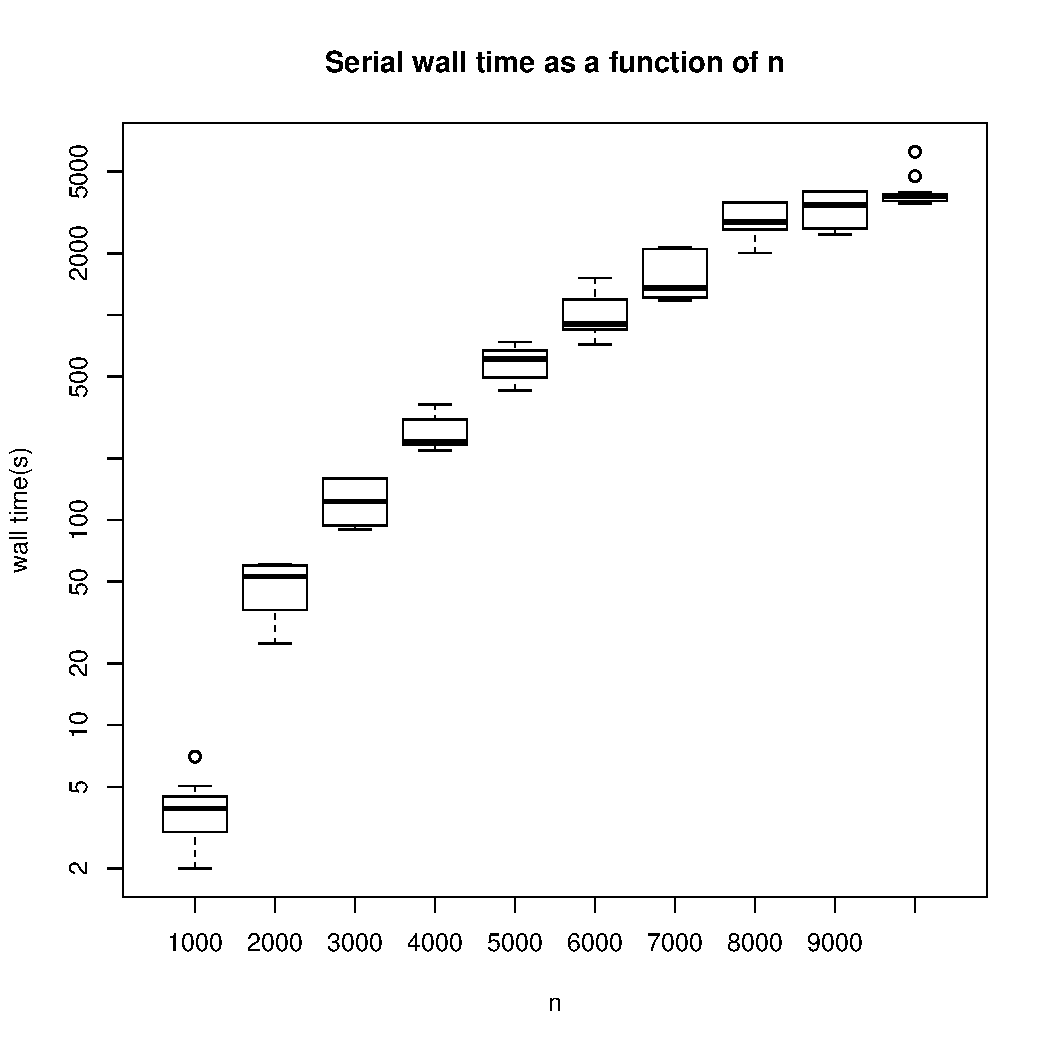
\includegraphics[width=12cm]{../analysis/serial_walltime.pdf}
  \end{center}
  \caption{Sequential implementation wall time as a function of problem size run on a single core.}
  \label{serial_walltime}
\end{figure}

\subsection{Parallel implementation wall time}
\begin{figure}[H]
  \begin{center}
    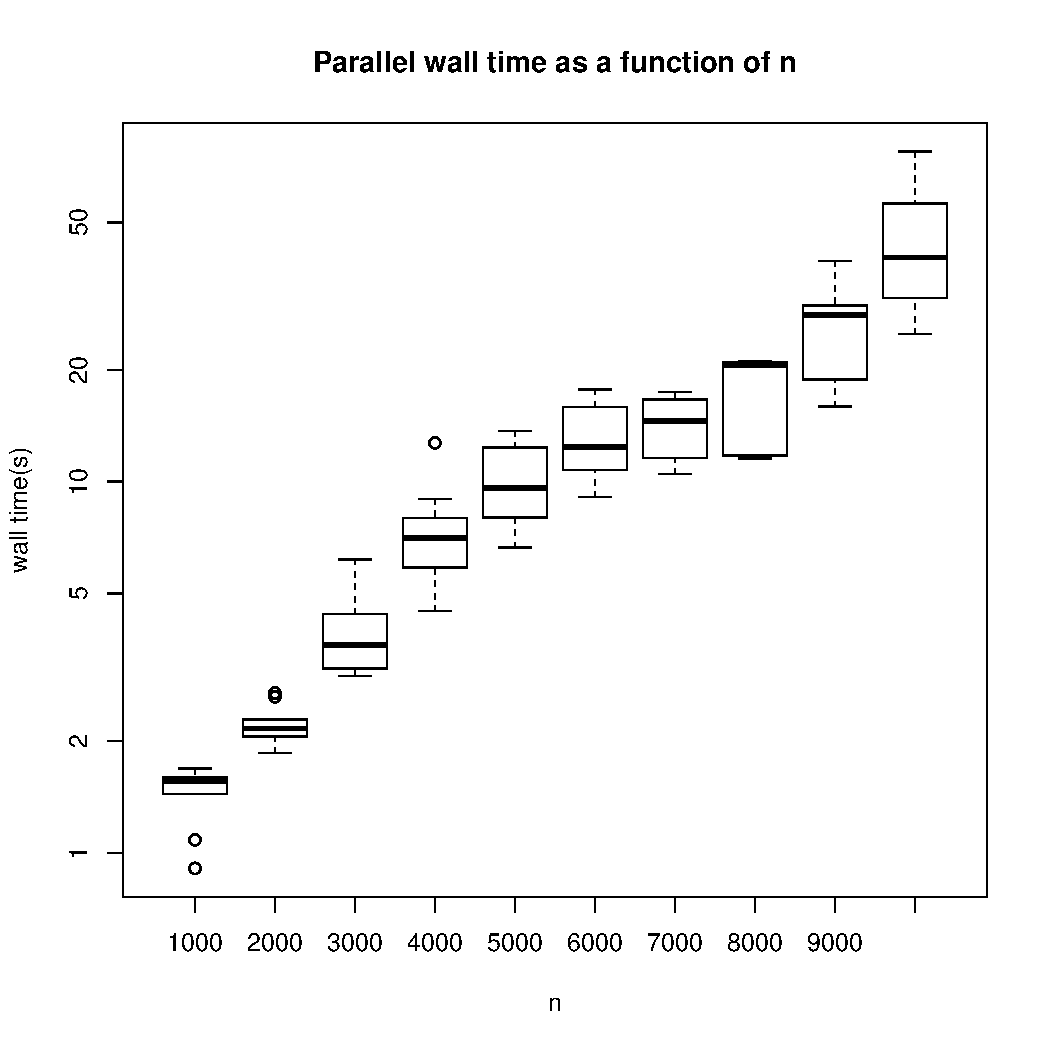
\includegraphics[width=12cm]{../analysis/parallel_walltime1.pdf}
  \end{center}
  \caption{Parallel implementation wall time as a function of problem size. Run on 5 nodes each with 5 MPI processes and 10 cores.}
  \label{parallel_walltime1}
\end{figure}

\begin{figure}[H]
  \begin{center}
    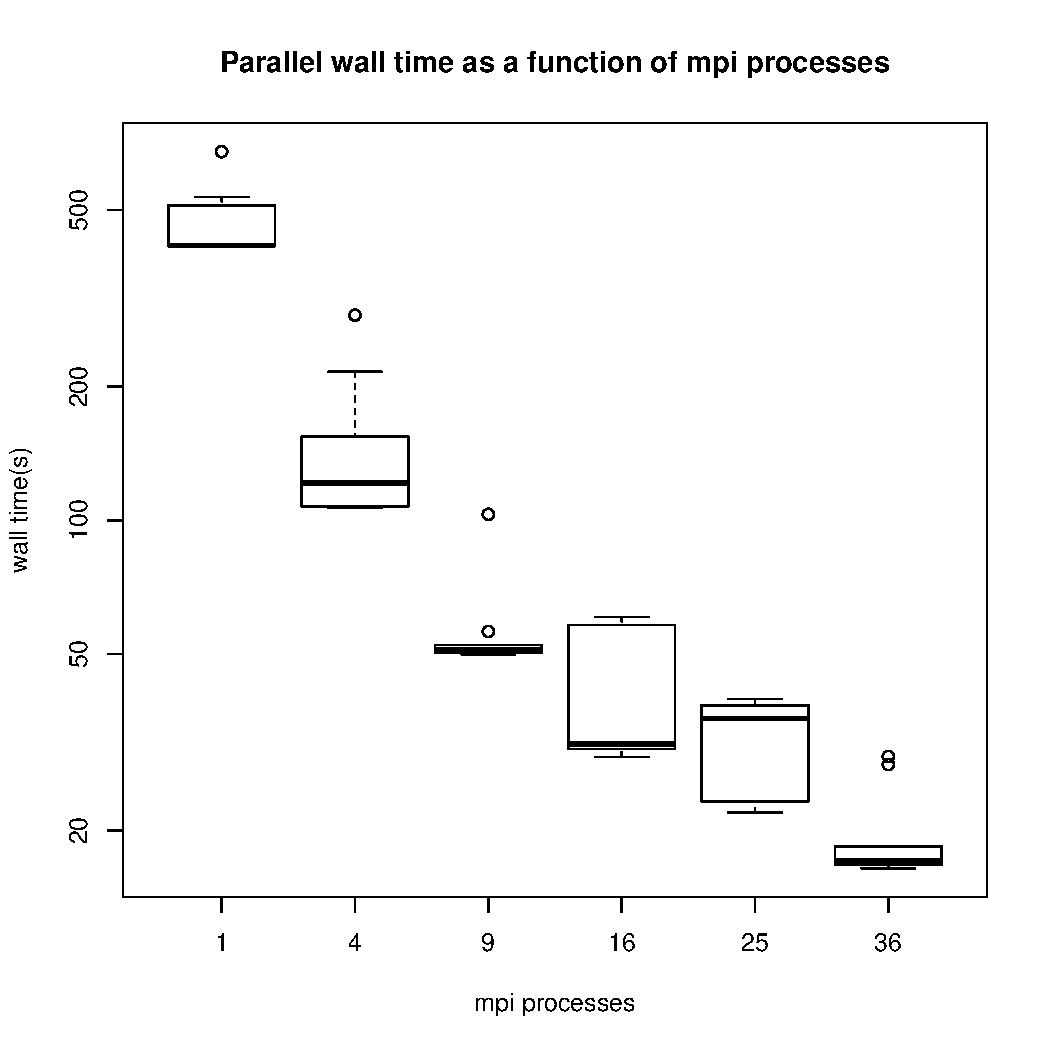
\includegraphics[width=12cm]{../analysis/mpi_nodes_walltime.pdf}
  \end{center}
  \caption{Parallel implementation wall time on a constant size problem, $n=10000$, as a function of mpi processes. For each mpi process there where two cores.}
  \label{parallel_walltime2}
\end{figure}

\subsection{Speedup}
\begin{figure}[H]
  \begin{center}
    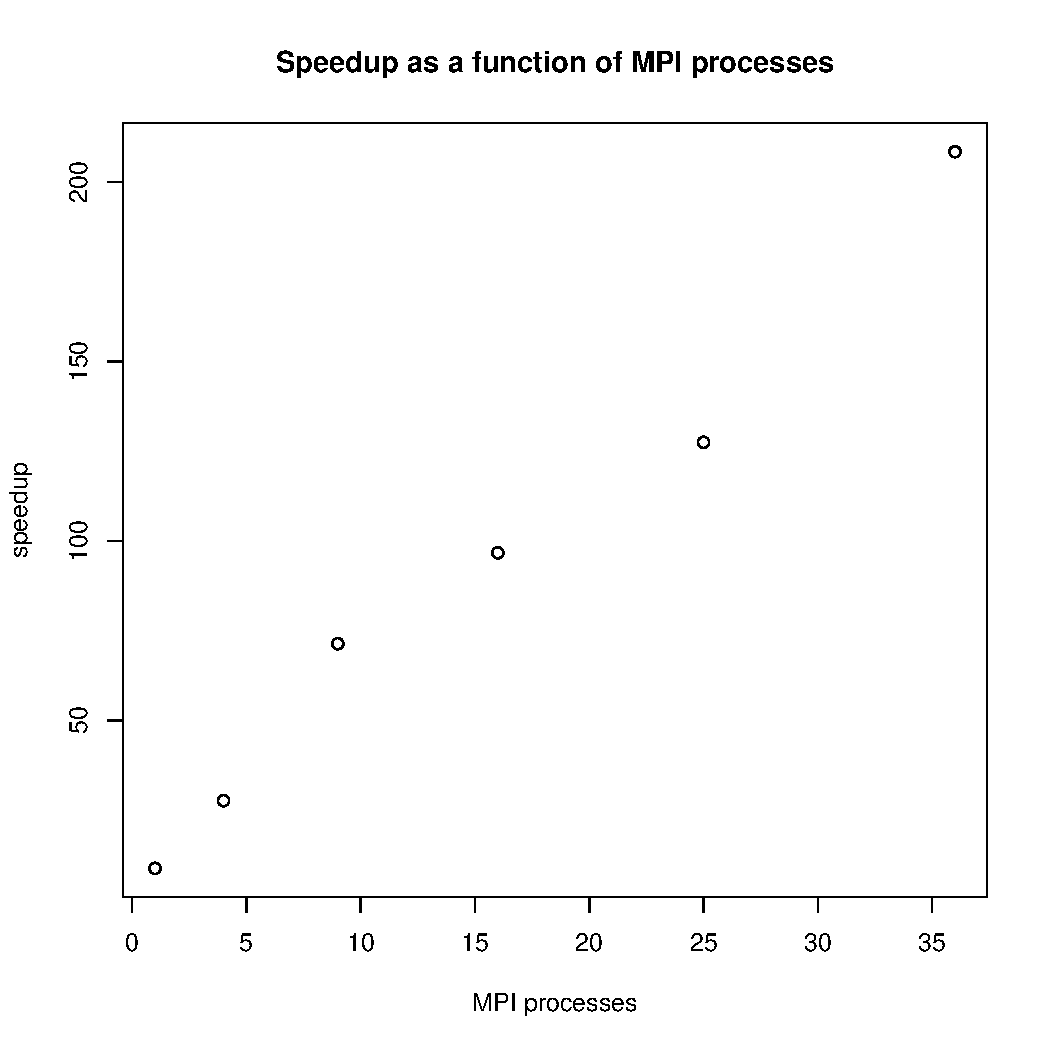
\includegraphics[width=12cm]{../analysis/mpi_nodes_speedup.pdf}
  \end{center}
  \caption{Speedup of program as a function of MPI processes when running on a constant problem size $n=10000$. For each MPI process there where two cores allocated to let OpenMP paralellize on the second core.}
  \label{mpi_nodes_speedup}
\end{figure}

\begin{figure}[H]
  \begin{center}
    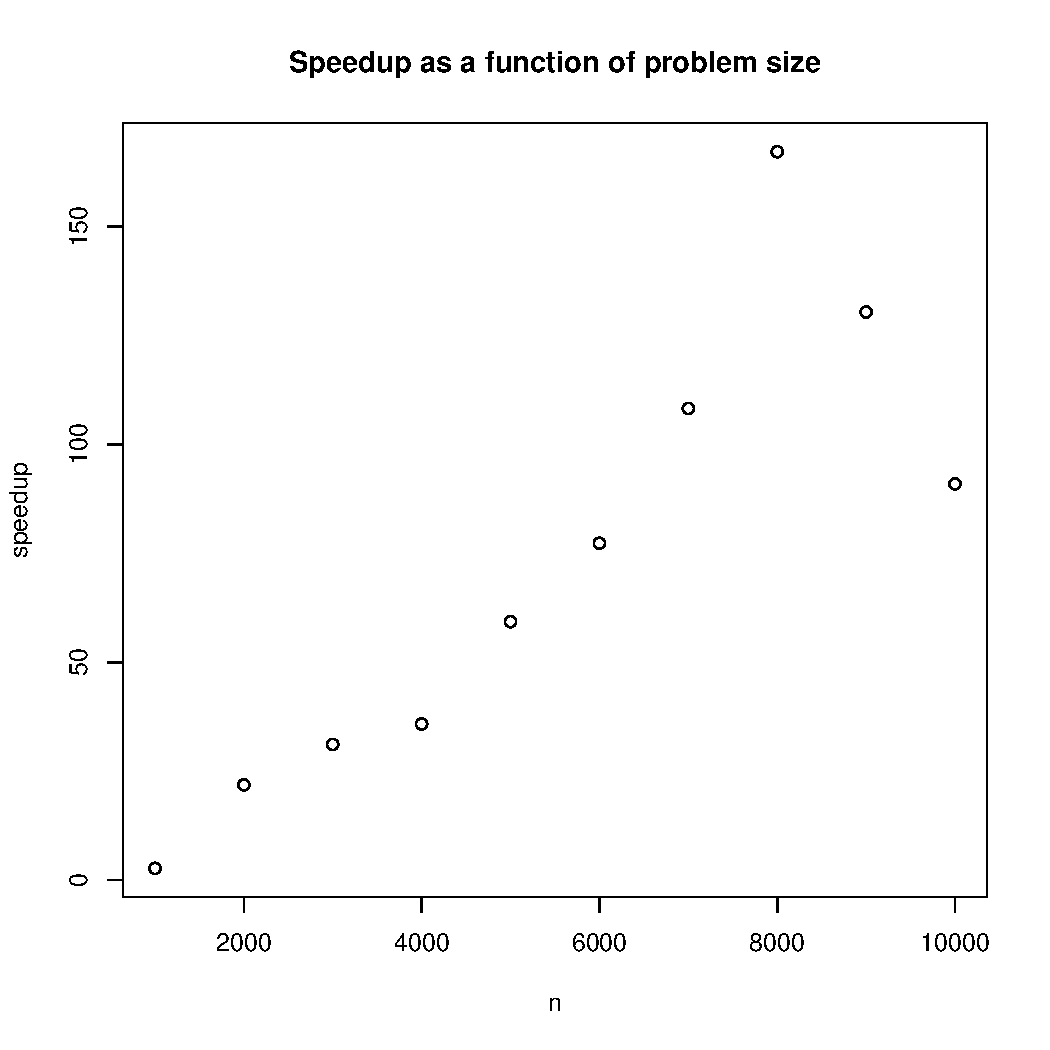
\includegraphics[width=12cm]{../analysis/problem_size_speedup.pdf}
  \end{center}
  \caption{Speedup of program as a function of problem size when running on a constant number of nodes, 5, MPI processes, 25, and cores, 50.}
  \label{problem_size_speedup}
\end{figure}

\section{Discussion}
From the speedup graphs \ref{mpi_nodes_speedup}, \ref{problem_size_speedup} there seems to be an almost unexplainable speedup running on
multiple cores.
\subparagraph{Speedup as a function of problem size}
To explain the speedup of around 160 the following factors has
to be taken into consideration.

5 nodes where used. Each node had
5 mpi processes and 10 cores available. The remaining 5 cores on each
node would be saturated by the paralellizm from the Intel MKL library.
All in all this adds up to 50 cores.

Secondly, the sequential implementation did not use any hardware dependent
optimizations. Most importantly the code was not vectorized. The parallel
implementation used MKL which for dgemm uses AVX2 instructions to do
4 double precition floating point operations at the same time. Because of
this up to 4 times the speedup can be claimed to come from vectorization.

Lastly and most importantly. The sequential implementation runs on one core. This
gives it acces to only that cores cache. Taking a closer look at the datasheet
for the E5-2670\cite{intel-datasheet} we observe that the cache hierarchy is
the following:
\begin{enumerate}
		\item L1 32kB instruction and 32kB data cache for each core
		\item L2 256kB shared instruction data cache for each core
		\item L3 20MB shared instruction data chache shared amongst all cores on the socket
\end{enumerate}
From a small calculation we see that for storing 3 1000x1000 matrices of doubles we need
\[
3 \times 1000^2 \frac{64}{8} = 3 \times 7.68 \text{Mb} = 22.89 \text{Mb}
\]
of memory.
Thus even the smallest problem, $n=1000$ will fill all the cache layers from L1 to L3.
For bigger problem this memory requirement increase on the order of $O(n^2)$.
When the chache is saturated the core will frequently have to go to RAM to get new parts of the problem. This memory
acces is several orders of magnitude slower that accessing the cache and the program sees a big
slowdown because of it.

Adding all these factors together, 50 cores, 4 times vectorization and at least 5 to 10 times slower memory access
gives numbers close to
\[
50 \times 4 \times 5 = 250 < \text{speedup} < 50 \times 4 \times 10 = 500.
\]
This means that without taking into account the syncronization overhead
the parallel algorithm could see between 250 and 500 times speedup in the given example.
The reason we are seeing about 160 is because
of all the syncronization introdused in the distributed algoritm.


\section{Journal}
\begin{enumerate}
	\item Started with Haskell. Managed to create a sequential that was on par with C and had much better readability and consiseness.
	\item Started looking at the accelerate library for Haskell. Managed to implement a matrix multiply in it but it lacked performance because of the non-flat nature of the matrix multiply algorithm in accelerate. This made it solver than a sequential C implementation.
	\item Contacted author of accelerate to see if there was any way to mend the problems but it turned out to be a limitation in the embedded language that accelerate is. There is no way to express the type of computation that matrix multiply is effeciently. This is because of the intermidiat dot-product you calculate when doing matrix multiply. Accelerate is extremely good at things that it's made for, like stencil computations. This was also looked at but because the application was to be solving extremely large linear systems they would not fit in the memory of one GPU.
	\item First version of the SUMMA algorithm used FORTAN routines for the matrix multipyl and array copying. Since FORTRAN ararys are column-major instead of row-major as in C this lead to unpredictable and really hard to debug problems in the algorithm.
	\item Scattering and gathering the matrices from the master node proved prone to error. Not because of bad libraries or programming errors. The challenge was creating the correct mapping in a general case from a contigous array to smaller blocked contigous arrays at the low abstraction level that C works.
	\item Implementing a really fast sequential version is not trivial since most of the tools for fast numerical code, BLAS, LAPACK etc. do paralellization without you knowing it. For example the first sequential version of the program used the cblas\_dgemm routine. When this routine was profiled it was experienced that the routine forked off several threads to do it's work, thus these library functions could not be used for a sequential implementation.
	\item Found out that increasing the number of cores available to the intel MKL compared to the number of MPI cores does not improve performance.
	\item TODO: write about the SUMMA algorithm - write about the above point - bundle up a script that is easy to run for submission - add a README to the code.
\end{enumerate}

\section{Mathematical derivation of solution method}
\label{sec:math_der}
Poisson's equation is given as
\[
-\Delta u = f
\]
where $\Delta = \nabla^2$ is the Laplace operator, u and f are real or complex valued functions in a
euclidian space. The equation is often written as
\[
-\nabla^2 u = f.
\]
In two dimensions the equation can be written as
\[
-\left( \frac{\partial^2}{\partial x^2} + \frac{\partial^2}{\partial y^2} \right) u(x,y) = f(x,y).
\]

This equation is continous and to work with it in the computer some discretized approximation has
to be made. This equation is continous and to work with it in the computer some discretized approximation has to be made. A finite difference approximation was chosen as it presents us with a
problem that have several solution strategies that illustrates well the important properties to
consider when designing parallel numerical algorithms.

After a FDM discretization we are left with a 2D regular grid. Each node in this grid represents
a point for which we compute an approximation to our functions $u(x,y)$ and $f(x,y)$.
Using a central difference approximation to the partial derivatives in each direction leaves us
with the following equation
\[
-\frac{u_{i+1,j}-2u_{i,j}+u_{i-1,j}}{h^2} - \frac{u_{i,j+1}-2u_{i,j}+u_{i,j-1}}{h^2} = f_{i,j}, 1\leq i,j \leq n-1.
\]

The goal is to express this 2D equation as a linear system of equations which we then can solve with
different techniques using the computer.

Let
\begin{equation}
       U = \begin{bmatrix}
               u_{1,1} & \dots & u_{1,n} \\
               \vdots  &       & \vdots \\
               u_{n,1} & \dots & u_{n,n}
       \end{bmatrix}
\end{equation}
be the discretized version of $u$.

Let 
\begin{equation}
       T = \begin{bmatrix}
               2 & -1 & & & \\
               -1 & 2 & -1 & & \\
               & \ddots & \ddots & \ddots &\\
               & & -1 & 2 & -1\\
               & & & -1 & 2 \\
       \end{bmatrix}
\end{equation}
be the discrete partial double derivative operator.
Then,
\begin{align*}
       (TU)_{i,j} &= 2u_{i,j} - u_{i+1,j}, &i=1,\\
       (TU)_{i,j} &= 2u_{i,j} - u_{i+1,j} - u_{i-1,j}, &2 \leq i \leq n-2,\\
       (TU)_{i,j} &= 2u_{i,j} - u_{i-1,j}, &i=n-1.\\
\end{align*}
and thus,
\[
\frac{1}{h^2}(TU)_{i,j} \approx - \left(\frac{\partial^2 u}{\partial x^2}\right)_{i,j}.
\]
By the same argument
\[
\frac{1}{h^2}(UT)_{i,j} \approx - \left(\frac{\partial^2 u}{\partial y^2}\right)_{i,j}.
\]

Our finite difference scheme can thus be written as
\[
\frac{1}{h^2}(TU + UT)_{i,j} = f_{i,j}, \quad 1\leq i,j \leq n-1.
\]
Or
\[
\label{linsys}
TU + UT = G
\]
where
\begin{equation}
G = h^2 \begin{bmatrix}
               f_{1,1} & \dots & f_{1,n} \\
               \vdots  &       & \vdots \\
               f_{n,1} & \dots & f_{n,n}
       \end{bmatrix}
\end{equation}.

The $T$ matrix may be diagonalized
\[
T = Q \Lambda Q^\top
\]
where $\Lambda$ is a diagonal matrix and $Q Q^\top=I$, the identity matrix.
When we insert this expression for $T$ in \eqref{linsys} we get
\[
Q \Lambda Q^\top U + U Q \Lambda Q^\top = G.
\]
Multiplying from rigth with $Q$ and left with $Q^\top$ gives
\begin{align*}
&(Q^\top Q) \Lambda Q^\top U Q + Q^\top U Q \Lambda (Q^\top Q)\\
&= \Lambda Q^\top U Q + Q^\top U Q \Lambda = Q^\top G Q.
\end{align*}


\begin{thebibliography}{9}

\bibitem{summa}
  Robert A. van de Geijn and Jerrell Watts (1997)
  \emph{SUMMA: Scalable Universal Matrix Multiplication Algorithm}
  \url{http://www.netlib.org/lapack/lawnspdf/lawn96.pdf}
 
\bibitem{mkl}
  \url{http://software.intel.com/en-us/intel-mkl}

\bibitem{r-project}
  \url{http://www.r-project.org/}

\bibitem{haskell}
  \url{http://haskell.org}

\bibitem{accelerate}
  \url{http://hackage.haskell.org/package/accelerate}

\bibitem{blas}
  \url{http://www.netlib.org/blas/}

\bibitem{lapack}
  \url{http://www.netlib.org/lapack/}

\bibitem{intel-datasheet}
  \url{https://www-ssl.intel.com/content/dam/www/public/us/en/documents/datasheets/xeon-e5-v2-datasheet-vol-1.pdf}

\bibitem{boxplot}
  \url{http://en.wikipedia.org/wiki/Box_plot}

\end{thebibliography}

\end{document}

